\documentclass[11pt]{article}
\usepackage{fullpage}
\usepackage[osf]{mathpazo}
\usepackage{latexsym}
\usepackage{amsfonts}
\usepackage[margin=1.2in]{geometry}
\usepackage{color}
\usepackage{graphicx}
\usepackage{subfigure}
\definecolor{webred}{rgb}{0.5,0,0}
\definecolor{webblue}{rgb}{0,0,0.7}
\definecolor{webdeepblue}{rgb}{0,0.3,0.9}
\usepackage[pdftex,colorlinks,citecolor=webblue,linkcolor=webdeepblue,urlcolor=webblue]{hyperref}

\newcommand{\ignore}[1]{}

%MARGIN TRICKS
\ignore{ \setlength{\textwidth}{17.6cm}
\setlength{\textheight}{23.cm} \setlength{\oddsidemargin}{-.2cm}
\setlength{\evensidemargin}{-.2cm} \setlength{\topmargin}{-.2cm}
\setlength{\headheight}{0cm} \setlength{\headsep}{-.2cm}
\setlength{\footskip}{1cm}
} %IGNORE


%\ignore{
%\setlength{\topmargin}{-1.2in}
%\setlength{\textheight}{23.0cm}
\setlength{\textwidth}{17.8cm} \setlength{\textheight}{23.2cm}
\setlength{\oddsidemargin}{-.4cm} \setlength{\evensidemargin}{-.4cm}
\setlength{\topmargin}{-.4cm} \setlength{\headheight}{-.3cm}
\setlength{\headsep}{0cm} \setlength{\footskip}{.8cm}
%} %IGNORE

%jpeg2ps  jpeg->eps
%subfigure...
%\begin{figure}
%\includegraphics[width=3in]{bcde}
%\caption{test}
%\end{figure}
%\begin{figure}
%\includegraphics[width=3in]{bcde}
%\caption{test}
%\end{figure}

%\date{\vspace{-1cm}}


%\vspace{-1cm}

\begin{document}
\title{%\vspace{-1cm}
{\sc Curriculum Vitae}}

\author{Limin Wang}

\date{\vspace{-.2cm}}

%%%%%%%%%%%%%%%%%%%%%%%%%%%%%%%%%%%%%
% Macros for this paper
% BKMRK 0
%%%%%%%%%%%%%%%%%%%%%%%%%%%%%%%%%%%%%


%\setcounter{page}{0}
\maketitle

%\vspace{-1.4cm}
\section*{Contact Information}
%\vspace{-.2cm}
\hspace{.52cm}Address: Institute of Information Engineering, Chinese Academy of Sciences

\hspace{1.54cm}C8 YiYuan, 80 XingShiKou Road

\hspace{1.54cm}Haidian District

\hspace{1.54cm}Beijing 100195

\hspace{1.54cm}P.R. China


Homepage: \href{http://csuncle.com/about/}{\tt http://csuncle.com}

%E-mail: \href{mailto:fan.terry.zhang@gmail.com}{\tt fan.terry.zhang@gmail.com}
\vspace{.2cm}
Tel: \href{(+86)156-0081-8233}{\tt (+86)156-0081-8233}
\vspace{.2cm}

E-mail: \href{wanglimin@iie.ac.cn}{\tt wanglimin@iie.ac.cn}

\hspace{1.40cm}\href{wlmnzf@hotmail.com}{\tt wlmnzf@hotmail.com}

%Cell: (+86)-13967175420; (+65)-86221742


%\vspace{-.2cm}
\section*{Research Interests}

Hardware Vulnerabilities, Computer Architecture, Side-channel Attacks, Model Checking

\section*{Education Background}
\hspace{.6cm}{09/2013-06/2017

B.E. in Computer Science and Technology,

School of Computer Science and Technology,

{\bf Hangzhou Dianzi University}, Hangzhou, China \\


 09/2017-Present 

M.S. in Computer Technology, 

School of Cyber Security,

{\bf University of Chinese Academy of Sciences}, Beijing, China

Advisor: { Professor  Dan Meng}

%Proficient and frequent user of C,C++,Matlab,Verilog
%
%Proficient in PCB Design,Altium Designer,Pspice
%
%Capable of utilizing AutoCAD,ADS

\section*{Publication} \label{paper}

\begin{enumerate}	
	\item {\bf Limin Wang}, Ziyuan Zhu*, Zhanpeng Wang, and Dan Meng. Analyzing The Security of The Cache Side Channel Defences With Attack Graphs. In Proceedings of the 25th Asia and South Pacific Design Automation Conference (ASP-DAC 2020), 2020. {\color{red}(Best Paper Candidate)} \href{http://csuncle.com/uploads/About/ASPDAC2020-final.pdf}{\tt [Download]}
	
	\item {\bf Limin Wang}, Ziyuan Zhu*, Zhanpeng Wang, and Dan Meng. Colored Petri Net Based Cache Side Channel Vulnerability Evaluation. in IEEE Access, vol. 7, pp. 169825-169843, 2019.\hspace{0.9cm}\href{http://csuncle.com/uploads/About/IEEE-Access-Print.pdf}{\tt [Download]}
	
\end{enumerate}

\section*{Awards}
%\vspace{-.2cm}

\begin{itemize}
	\item 2019, Merit/Triple A Student, University of Chinese Academy of Sciences, China
	\item 2017, Outstanding Graduates, Hangzhou Dianzi University, China
	\item 2015, Merit/Triple A Student, Hangzhou Dianzi University, China
	\item 2015, The Second-class Scholarship for Outstanding Students, Hangzhou Dianzi University, China
	\item 2015, The First-class Scholarship for Outstanding Students, Hangzhou Dianzi University, China
	\item 2014, Outstanding Student Leader Award, Hangzhou Dianzi University, China
	\item 2014, Merit/Triple A Student, Hangzhou Dianzi University, China
	\item 2014, The First-class Scholarship for Outstanding Students, Hangzhou Dianzi University, China
	
	{\bf NOTE:} The scanned copies of certificates are attached in the \textbf{Attachments}.
\end{itemize}


\section*{Research Experience}

\begin{itemize}

\item {\bf Memory security}\\
\vspace{-.3cm}

$\cdot$ Propose a new algorithm for ORAM, the algorithm can make ORAM hide the data access pattern at a lower cost. The ORAM module with the new algorithm has been implemented on the Gem5 simulator, and the research results were submitted to ICCD 2018. I collaborated this work with Zhanpeng Wang in the Institute of Information Engineering. 
\end{itemize}

\begin{itemize}
\vspace{-.3cm}

\item {\bf Security analysis of defenses for hardware vulnerabilities and cache attacks}\\
\vspace{-.3cm}

$\cdot$ Modify the open source model checker NuSMV so that it can generate multiple counterexamples.\\
\vspace{-.3cm}

$\cdot$ Propose a new method to analyze the security of the side channel defenses. Formal methods (model checking) are introduced in our method to make it more rigorous and the attack graph technology can also help simplify the counterexamples generated by model checker and make counterexamples easier to analyze. The research has been published at ASP-DAC 2020.
\end{itemize}


\begin{itemize}
\item {\bf Quantitative analysis of cache side channel risk }\\
\vspace{-.3cm}

$\cdot$ Propose a new model based quantitative method to evaluate the threat of different cache side channel attacks and hardware vulnerabilities in the computer environment with different security mechanisms. To make our evaluation approach more reasonable, in addition to the attack method, we also consider both the conditions on which the attack steps depend and the differences of attack capability among different attacks. In this research, \emph{Common Vulnerability Scoring System (CVSS)} is adopted to score the attack power of each attack step as the weight, we also analyze the attack methods and their requirements to obtain the probability of success of every attack step. The attack steps and both the probability and weight will finally be modeled as a three-step colored Petri net model. The research results have been published by IEEE Access. \\
\end{itemize}


\section*{Other Experience}
%\vspace{-.2cm}
\begin{itemize}

\item 08/2018 -- Present. Worked in the Computer Architecture Security Lab, Institute of Information Engineering, Chinese Academy of Sciences. \\
Advisor: Prof. Dan Meng

\item 11/2015 -- 06/2017. Worked as an intern on a face recognition project in the Institute of Image \& Graphs, Hangzhou Dianzi University. \\
 Advisor: Prof. Jianjun Li
 
\item 06/2014 -- 09/2015. Worked as a full stack developer in Geese Technology Ltd, Hangzhou. \\
 Noted: Geese Technology Ltd is a startup company which was founded by my classmates, and I was one of the technical leaders who were invited early.
\end{itemize}



\section*{References}

\quad\,\,
\begin{tabular}{l}


{\bf Professor \href{http://people.ucas.ac.cn/~md}{Dan Meng}} (Advisor)\\
University of Chinese Academy of Sciences, Beijing, China  \\
E-mail: \href{mailto:mengdan@iie.ac.cn}{mengdan@iie.ac.cn}\\
\\

{\bf Professor \href{http://people.ucas.edu.cn/~0039297}{Ziyuan Zhu}}\\
University of Chinese Academy of Sciences, Beijing, China  \\
E-mail: \href{mailto:zhuziyuan@iie.ac.cn}{zhuziyuan@iie.ac.cn}\\
\\

{\bf Professor \href{https://person.zju.edu.cn/fanzhang}{Fan (Terry) Zhang}}\\
Zhejiang University, Hangzhou, China  \\
Tel:(+86)137-7735-6409 \\
E-mail: \href{mailto:fanzhang@zju.edu.cn}{fanzhang@zju.edu.cn}\\
\\

%\end{tabular}
\quad

\end{tabular}

\section*{Attachments} 
\label{section:sec_attach}

The scanned copies of my award certificates and transcripts are shown below.

\begin{figure}[ht]
	\centering
	% Requires \usepackage{graphicx}
	\includegraphics[scale=0.7]{fig/MS_transcript.JPG}\\
	\caption{Master's Transcript.}
\end{figure}
	
\begin{figure}[ht]
	\centering
	% Requires \usepackage{graphicx}
	\includegraphics[scale=0.7]{fig/BE_transcript.JPG}\\
	\caption{Undergraduate Transcript.}
\end{figure}

\begin{figure}[ht]
	\centering
	% Requires \usepackage{graphicx}
	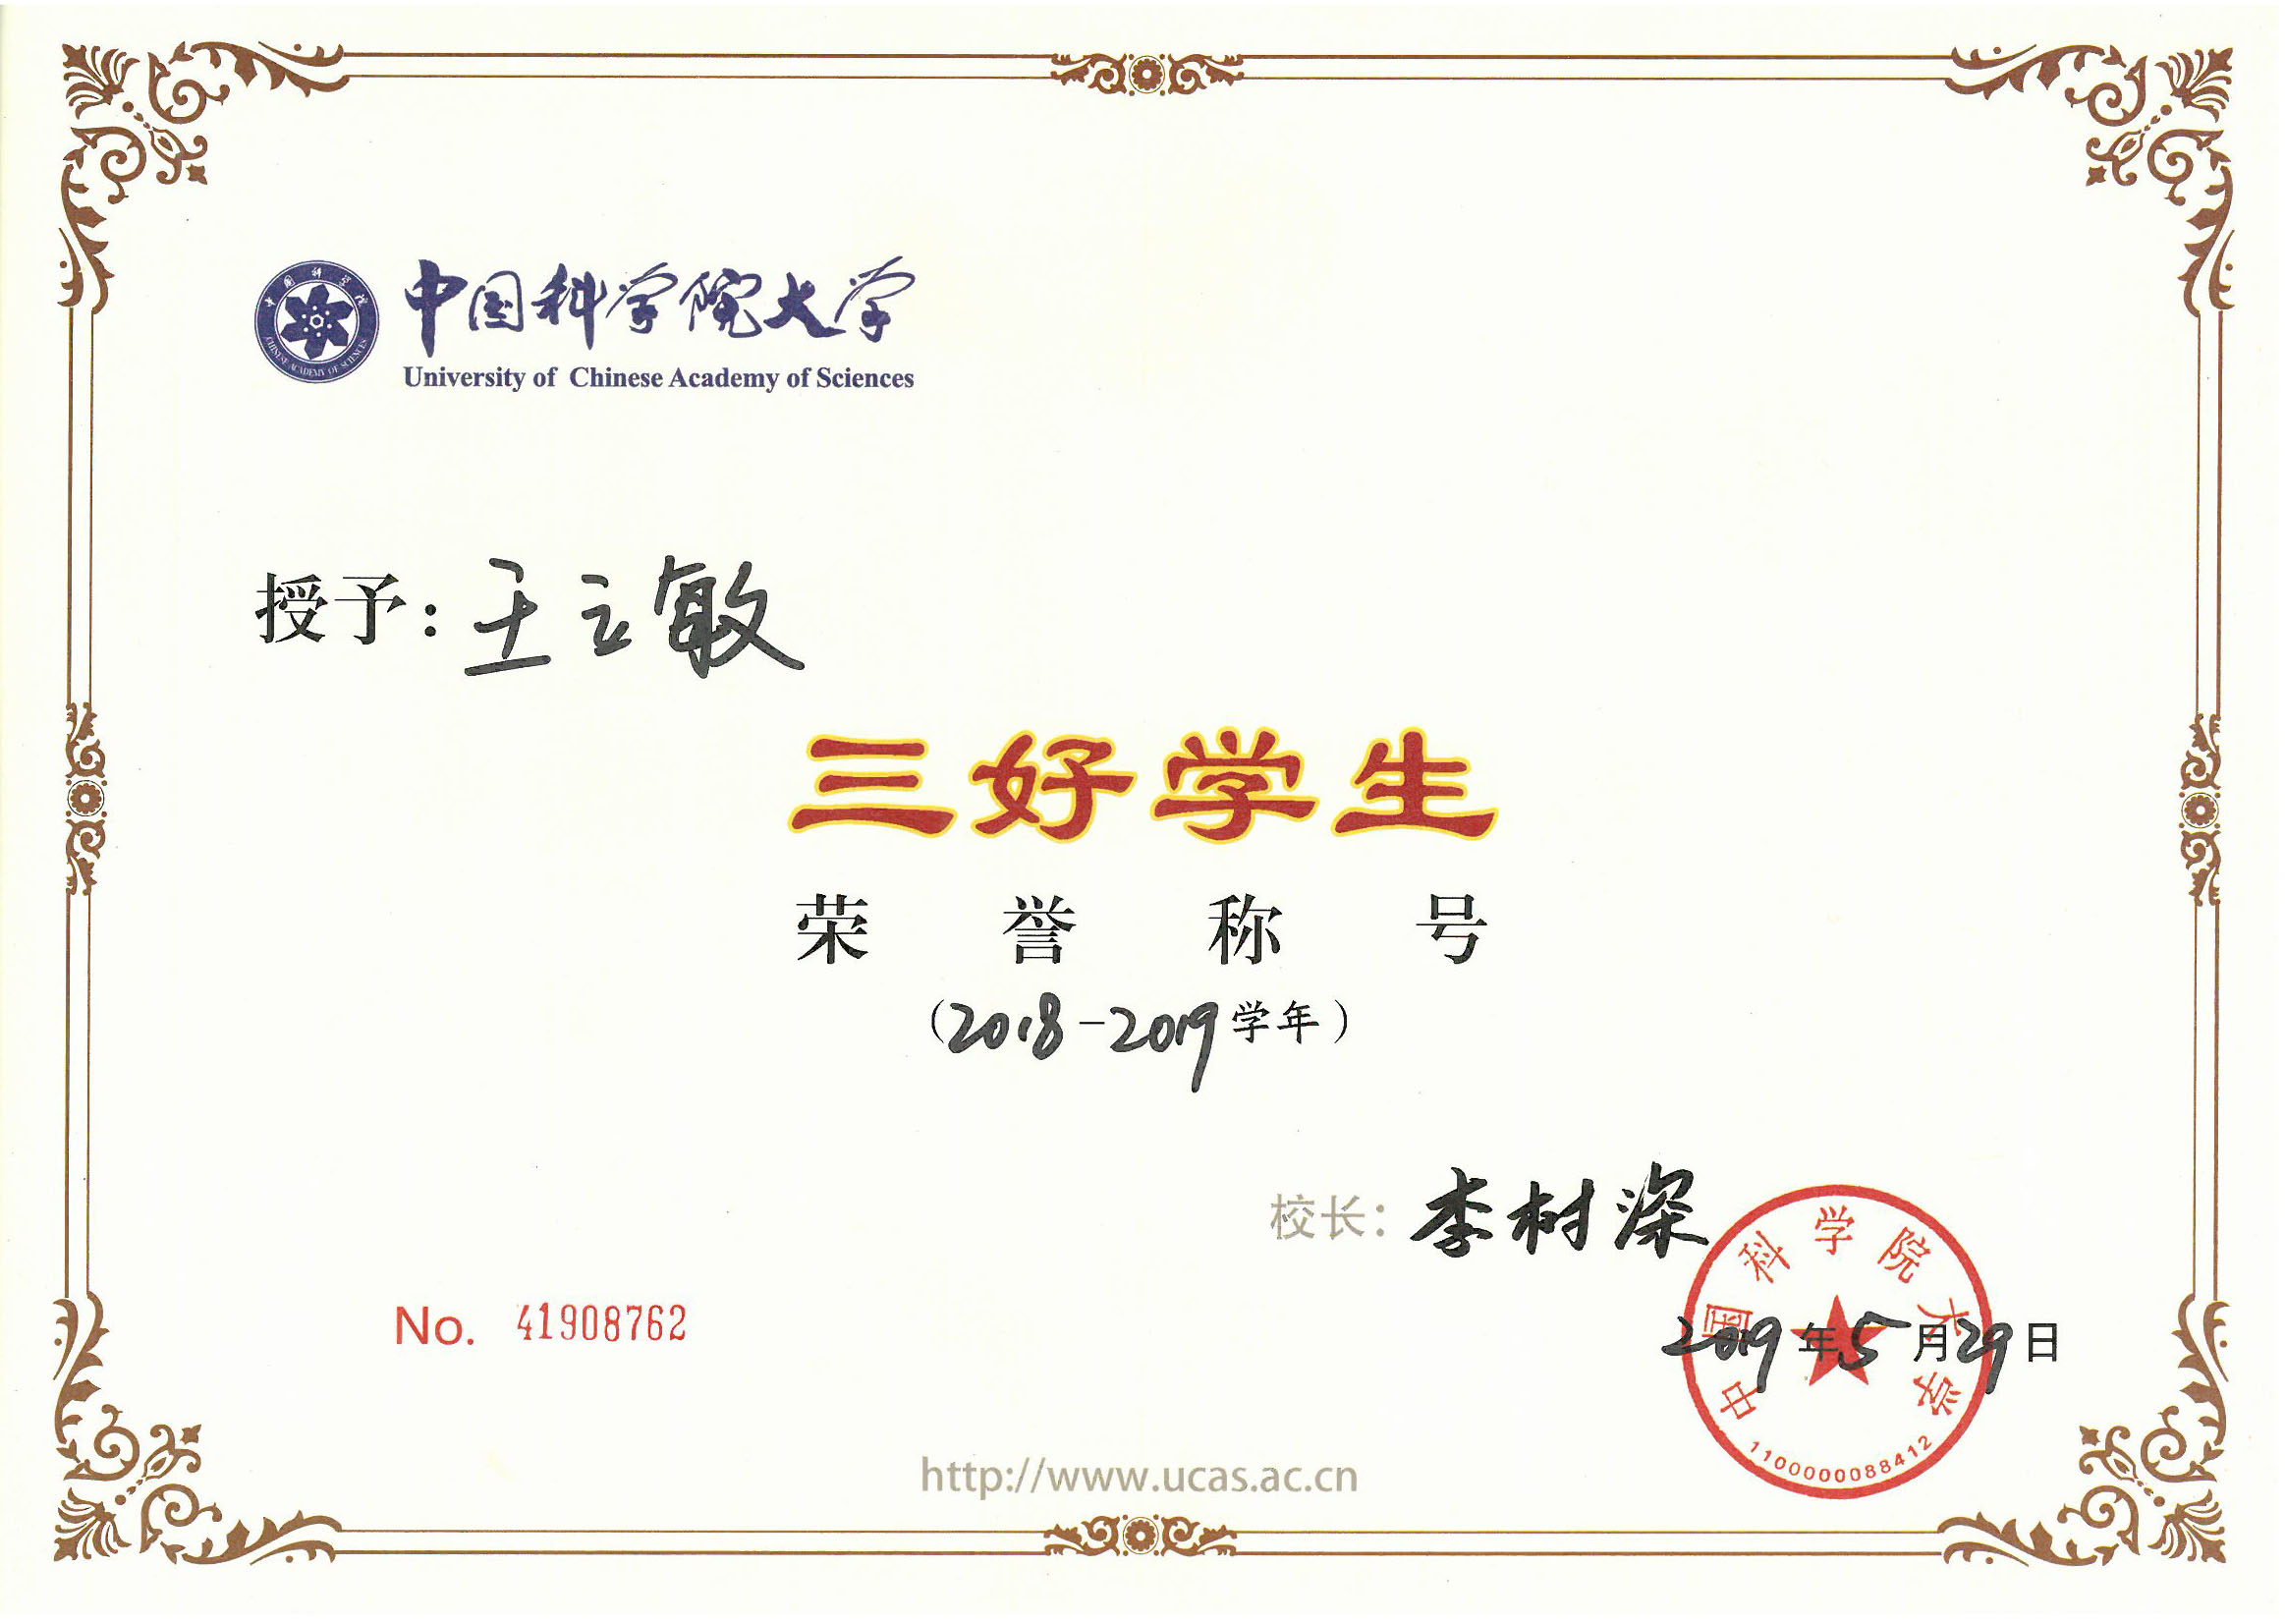
\includegraphics[width=14cm]{fig/cer1.jpg}\\
	\caption{2019, Merit/Triple A Student.}
\end{figure}

\begin{figure}[ht]
	\centering
	% Requires \usepackage{graphicx}
	
\includegraphics[width=14cm]{fig/cer2.jpg}\\
	\caption{2017, Outstanding Graduates.}
\end{figure}

\begin{figure}[ht]
	\centering
	% Requires \usepackage{graphicx}
	
\includegraphics[width=14cm]{fig/cer3.jpg}\\
	\caption{2015, Merit/Triple A Student.}
\end{figure}

\begin{figure}[ht]
	\centering
	% Requires \usepackage{graphicx}
	
\includegraphics[width=14cm]{fig/cer4.jpg}\\
	\caption{2015, The Second-class Scholarship for Outstanding Students.}
\end{figure}

\begin{figure}[ht]
	\centering
	% Requires \usepackage{graphicx}
	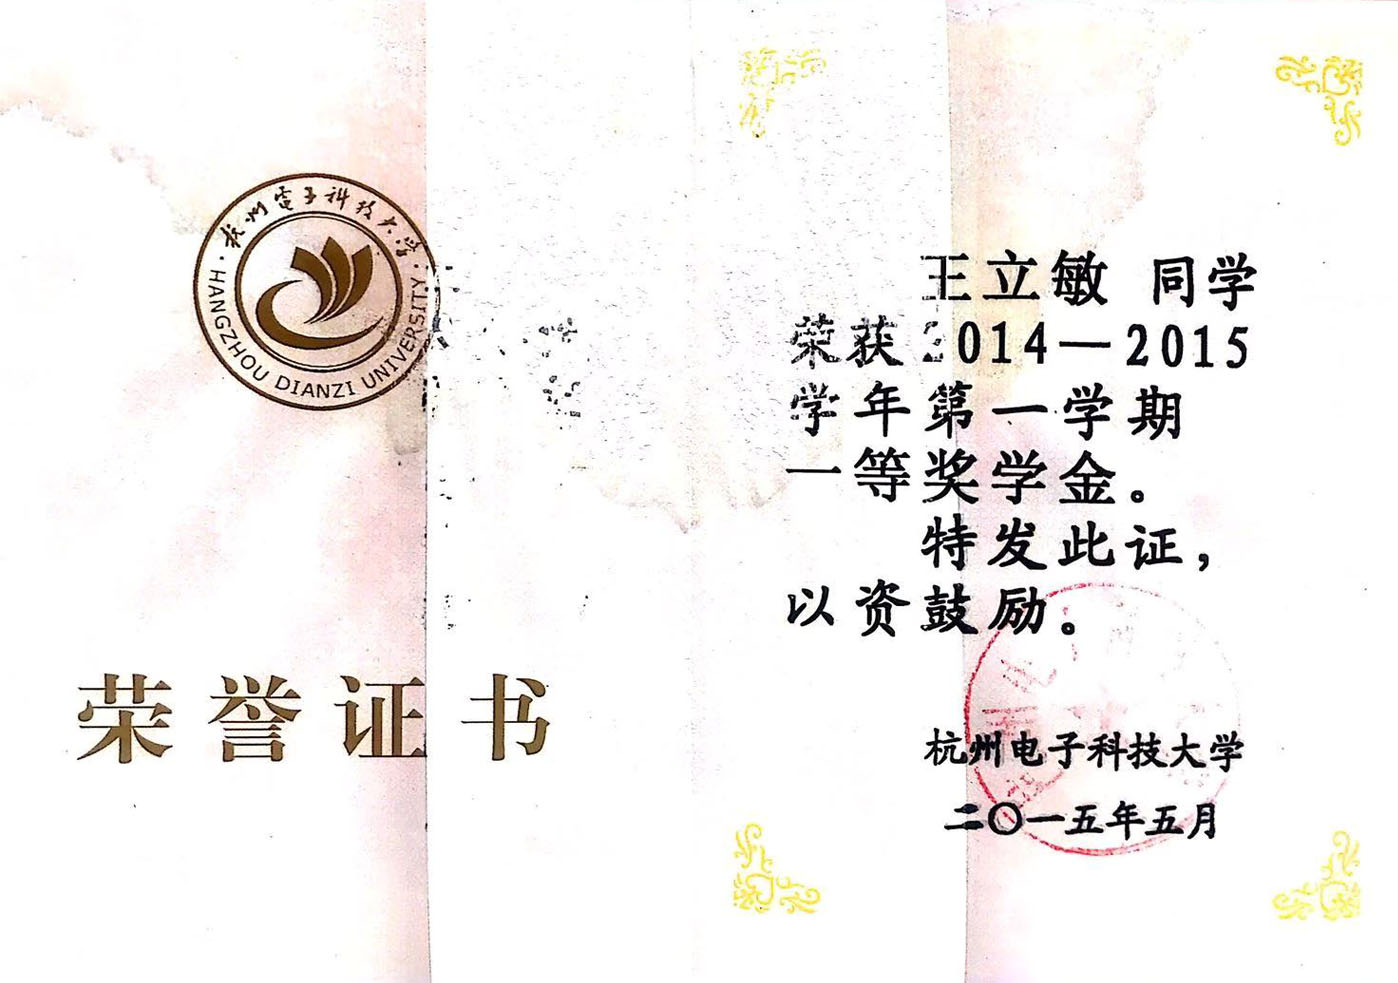
\includegraphics[width=14cm]{fig/cer5.jpg}\\
	\caption{2015, The First-class Scholarship for Outstanding Students.}
\end{figure}

\begin{figure}[ht]
	\centering
	% Requires \usepackage{graphicx}
	
\includegraphics[width=14cm]{fig/cer6.jpg}\\
	\caption{2014, Outstanding Student Leader Award.}
\end{figure}

\begin{figure}[ht]
	\centering
	% Requires \usepackage{graphicx}
	
\includegraphics[width=14cm]{fig/cer7.jpg}\\
	\caption{2014, Merit/Triple A Student.}
\end{figure}

\begin{figure}[ht]
	\centering
	% Requires \usepackage{graphicx}
	
\includegraphics[width=14cm]{fig/cer8.jpg}\\
	\caption{2014, The First-class Scholarship for Outstanding Students.}
\end{figure}
%\begin{figure}[ht]
%	\begin{center}
%		\subfigure[Samsung Scholarship.]{		
%			
\includegraphics[scale=0.35]{fig/cer3.jpg}}
%		\subfigure[Outstanding Graduate Leader Award.]{
%			
\includegraphics[scale=0.35]{fig/cer4.jpg}}
%		\subfigure[Graduate of Merit/Triple A graduate.]{
%			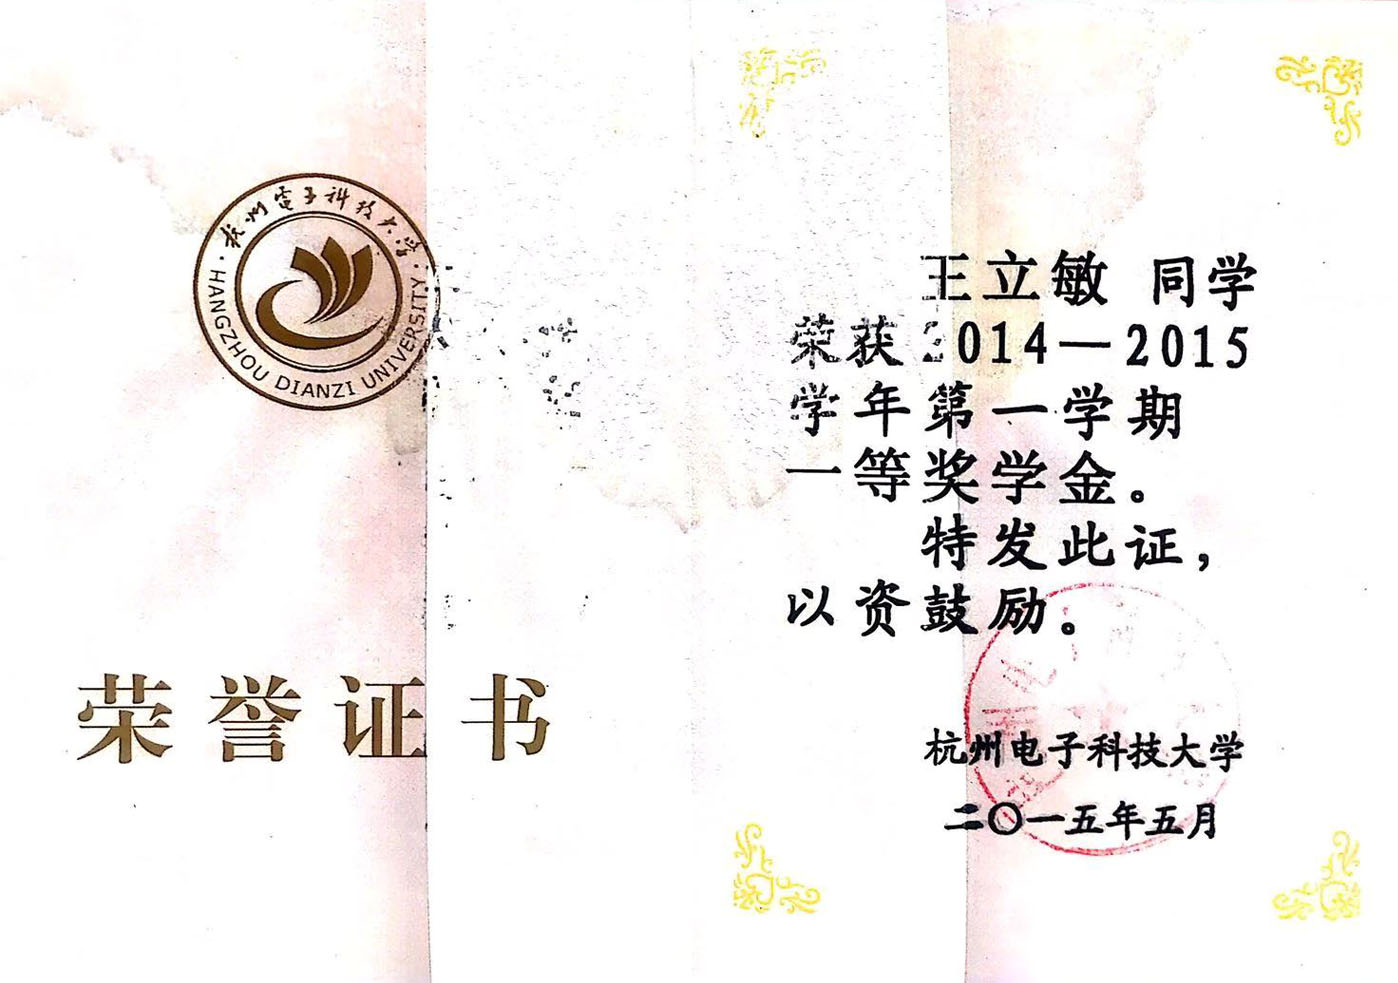
\includegraphics[scale=0.35]{fig/cer5.jpg}}
%		\subfigure[Award of Honor for Graduate.]{
%			
\includegraphics[scale=0.35]{fig/cer6.jpg}}
%	\end{center}
%	%\caption{}
%	\label{fig_dis} %% label for entire figure
%\end{figure}

%\begin{figure}[ht]
%	\begin{center}
%		\subfigure[The Third Prize of the National Talents Training Base.]{		
%			
\includegraphics[scale=0.35]{fig/cer7.jpg}}
%		\subfigure[The Third-class Scholarship for Outstanding Students.]{
%			
\includegraphics[scale=0.35]{fig/cer8.jpg}}
%		\subfigure[The Third-class Scholarship for Outstanding Merits.]{
%			
\includegraphics[scale=0.35]{fig/cer9.pdf}}
%	\end{center}
%	%\caption{}
%	\label{fig_dis} %% label for entire figure
%\end{figure}





\end{document}
